\documentclass[final]{beamer}

% ====================
% Packages
% ====================

\usepackage[T1]{fontenc}
\usepackage{lmodern}
\usepackage{pdfpages}

\usepackage[orientation=portrait, size=a2, scale=1.15]{beamerposter}
\usetheme{gemini}
\usecolortheme{nott}
\usepackage{graphicx}
\usepackage{booktabs}
\usepackage{tikz}
\usepackage{pgfplots}
\pgfplotsset{compat=1.14}
\usepackage{anyfontsize}
\setbeamercolor{headline}{bg=white}
\setbeamercolor{headline}{fg=black}

% ====================
% Length
% ====================

\newlength{\sepwidth}
\newlength{\colwidth}
\setlength{\sepwidth}{0.025\paperwidth}
\setlength{\colwidth}{0.45\paperwidth}

\newcommand{\separatorcolumn}{\begin{column}{\sepwidth}
\end{column}}

% ====================
% Title
% ====================

\title{\fontsize{23.25}{26}\selectfont Low-Cost, Low-Noise Lithium-Ion Battery
Power Supply for Enhanced Accessibility in Electronics Research}

\author{\normalsize Benjamin Datsko \inst{1} \and Luke Wormald \inst{2} \and
Michael Flynn \inst{3}}

\institute[shortinst]{\small Flynn Research Group, University of Michigan Department of Electrical and Computer Engineering}

% ====================
% Logo
% ====================

\logoright{
\includegraphics[height=4cm]{University-Of-Michigan-Logo.png}\hspace{20pt}}
\logoleft{\hspace{20pt}
\includegraphics[height=2.5cm]{SRC_Logo_Emblem-Name_CMYK.jpg}}

% ====================
% Body
% ====================

\begin{document}
	\begin{frame}[t]
		\begin{columns}[t]
			\separatorcolumn

			\begin{column}{\colwidth}
				\begin{block}{Background}
					Developing low-cost, low-noise power supplies is crucial for enabling
					accessible, high-quality testing of sensitive integrated circuits in academic
					and research settings. This project aims to create a power supply that
					meets the following target specifications:
					\begin{itemize}
						\item Noise level: Less than 5 mV peak-to-peak.

						\item Cost: Under \$100.

						\item Performance: Comparable to or better than industry-standard
							power supplies.

						\item Features: Rechargeable, portable, and safe.
					\end{itemize}

					By leveraging lithium-ion batteries, this device achieves low-noise characteristics
					while maintaining affordability.
				\end{block}

				\begin{block}{Approach}
					\begin{figure}
						\centering
						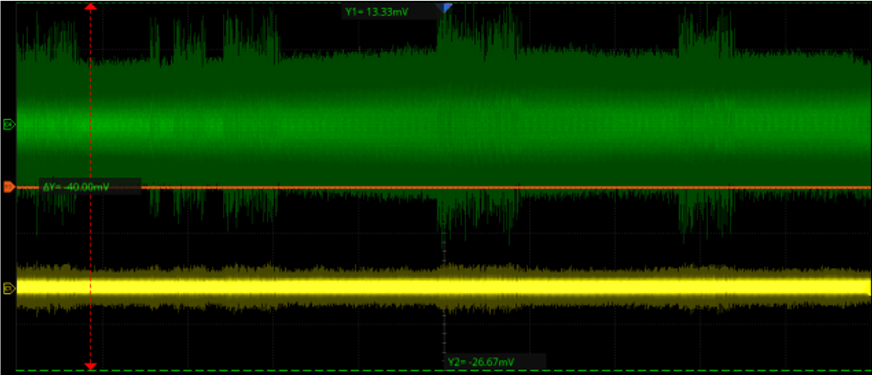
\includegraphics[width=.92\textwidth]{noise_compare2.png}
						\caption{5V signal Agilent E3631A (top) versus battery solution (bottom)}
					\end{figure}

					This design comprises a motherboard and a daughterboard, where the daughterboard
					enables user interaction with the GUI via buttons, and the motherboard
					contains all remaining logic.

					\textbf{Key Features:}
					\begin{itemize}
						\setlength{\itemsep}{0pt}
						\setlength{\parskip}{0pt}

						\item \textbf{Power Source:} Two 18650 Li-Ion (Lithium Ion) cells in
							series for stable, low-noise power without AC or DC switching conversion.

						\item \textbf{Microcontroller:} 8-bit AVR-based ATMEGA32U chip for
							efficient control of power management and user interface (UI)
							running Real-Time Operating System (RTOS) and Battery Protection
							System (BPS).

						\item \textbf{Safety Features:} Cell voltage/temperature monitoring,
							passive balancing, over-current protection.

						\item \textbf{Output Control:} Conditional logic block using PFETs
							and NFETs with a relay for battery recharge/discharge.

						\item \textbf{User Interface:} OLED display, LED indicator,and navigation
							buttons for interacting with the control panel GUI.
					\end{itemize}

					\textbf{Board Layout Strategies for Noise Reduction:}
					\begin{itemize}
						\setlength{\itemsep}{0pt}
						\setlength{\parskip}{0pt}

						\item 2-layer board with thick power traces and isolated signal lines.

						\item Low-pass filter and ferrite beads for high/low-frequency filtering.

						\item Careful component selection (SMD, temperature-stable capacitors,
							e.g. X7R).
					\end{itemize}

					\vspace{-0.5em}
					\textbf{Performance Analysis Device:} Siglent SDS2204X oscilloscope.

					\begin{figure}
						\fbox{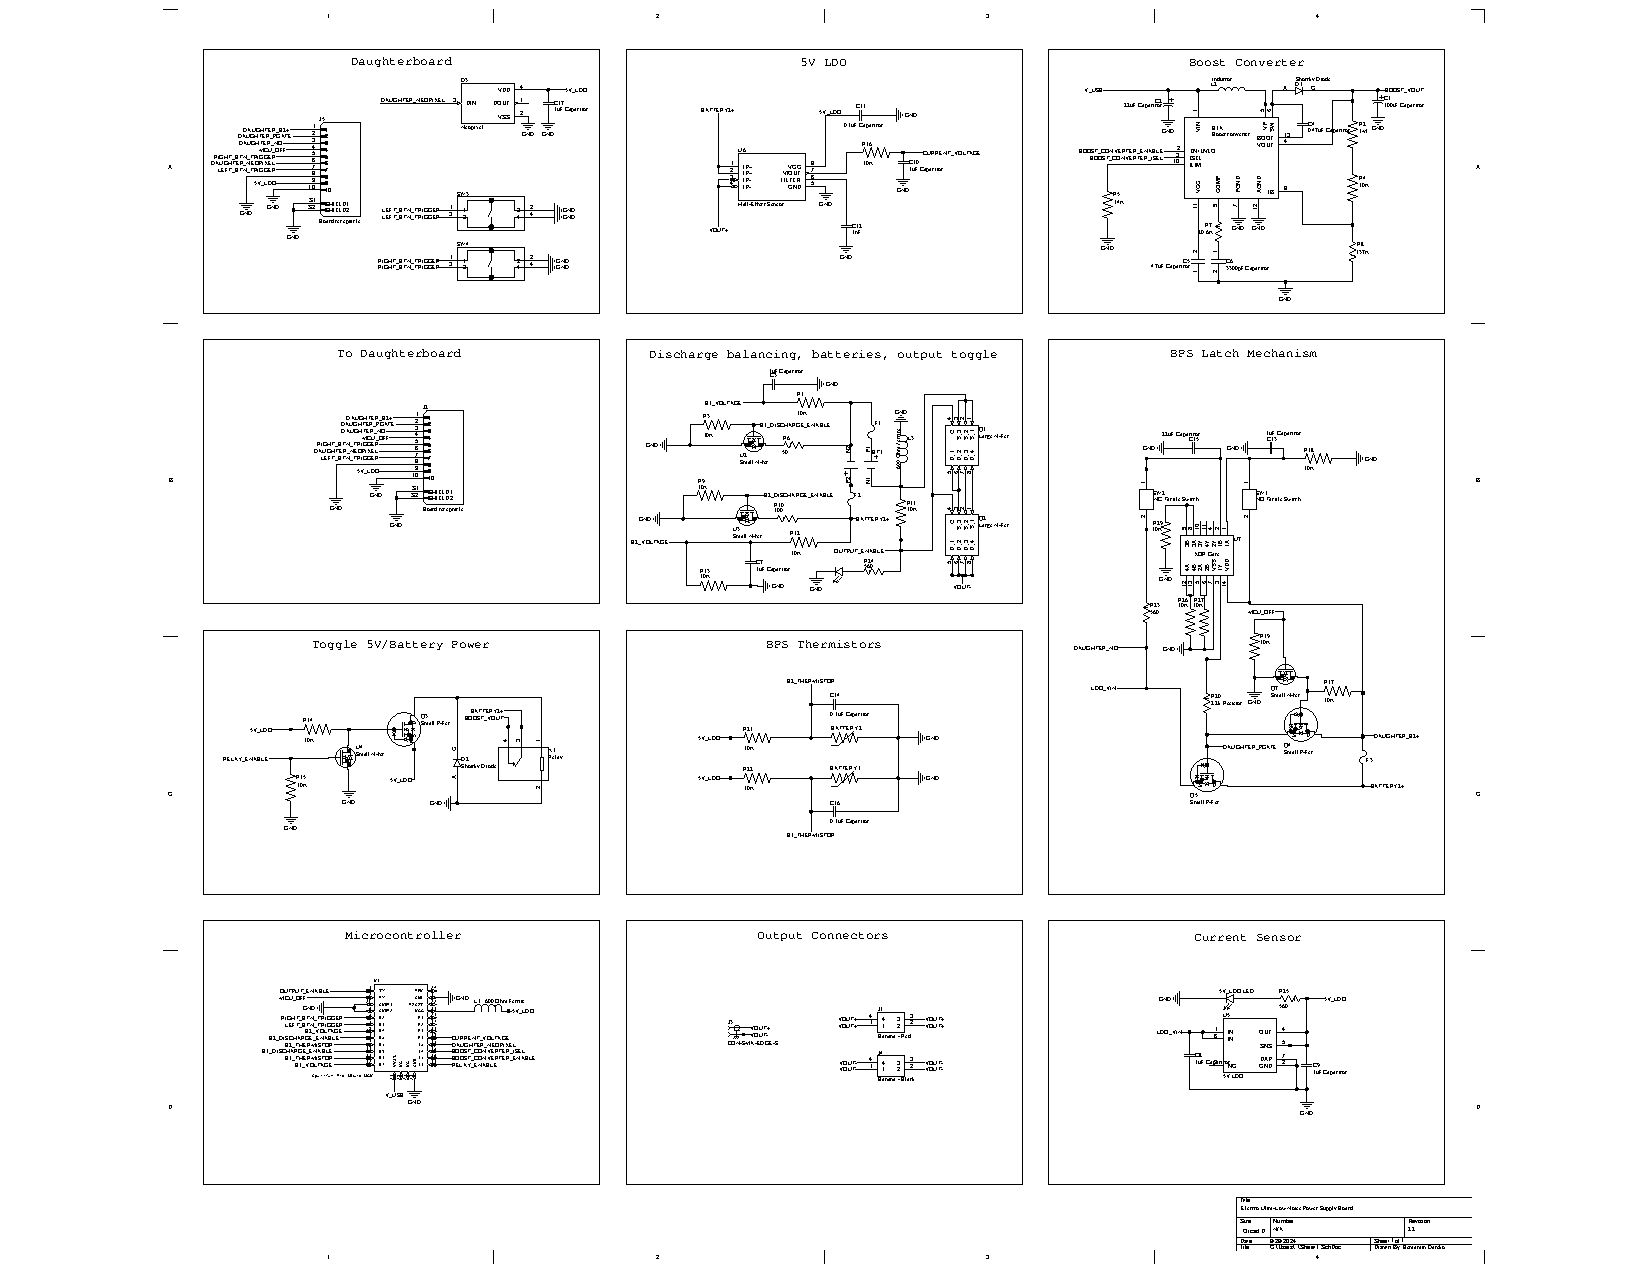
\includegraphics[width=.92\textwidth, page=1]{
							meowschematic.pdf
						}}
						\caption{System schematic}
					\end{figure}
				\end{block}
			\end{column}

			\separatorcolumn

			\begin{column}{\colwidth}
				\begin{block}{Results}
					\begin{figure}
						\begin{minipage}[t]{0.47\textwidth}
							\includegraphics[
								width=\textwidth,
								height=0.90\textheight,
								keepaspectratio
							]{motherboard2.png}
						\end{minipage}
						\hfill
						\begin{minipage}[t]{0.49\textwidth}
							\raisebox{185pt}[\height][0pt]{%
							\begin{minipage}{\textwidth}
								\begin{subfigure}
									{\textwidth}
									\includegraphics[
										width=\textwidth,
										height=0.315\textheight,
										keepaspectratio
									]{daughterboardtop2.png}
								\end{subfigure}
								\vspace{0.01\textheight}
								\begin{subfigure}
									{\textwidth}
									\includegraphics[
										width=\textwidth,
										height=0.315\textheight,
										keepaspectratio
									]{daughterboardbottom2.png}
								\end{subfigure}
								\vspace{0.01\textheight}
								\begin{subfigure}
									{\textwidth}
									\includegraphics[
										width=\textwidth,
										height=0.315\textheight,
										keepaspectratio
									]{container2.png}
								\end{subfigure}
							\end{minipage}
							}
						\end{minipage}
						\centering
						\caption{Motherboard (left), daughterboard (top right), and system
						in 3D printed case (bottom right)}
					\end{figure}

					When a 50 ohm load resistor is applied, the power supply exhibits a noise
					level of 3.89 mV peak-to-peak. Compared to the average noise of a sample of bench power
					supplies used in laboratory settings, the battery supply measures \textbf{
					40\% lower }:

					\begin{table}
						\centering
						\begin{tabular}{lcc}
							\toprule Power Supply      & Noise (mV)    & Price (\$)  \\
							\midrule Agilent E3631A    & 6.41          & 1,414       \\
							Keysight E36103B           & 7.11          & 828         \\
							Siglent SPD3303X-E         & 6.53          & 469         \\
							Rigol DP832                & 7.02          & 529         \\
							\textbf{Proposed Solution} & \textbf{3.89} & \textbf{80} \\
							\bottomrule
						\end{tabular}
						\caption{Power supply noise (mV Pk-Pk) and associated price (USD)}
					\end{table}
				\end{block}

				\begin{block}{Technology Transfer and Impact}
					This compact, low-noise lithium-ion battery power supply is ideal for
					powering sensitive electronic test benches, such as those used for neuromorphic
					computing ICs and CMOS Ising solvers. With noise levels as low as 3.89
					mV peak-to-peak and an adjustable voltage range of 5V to 8.4V, it
					ensures the integrity of noise-sensitive operations is maintained under test conditions, while also doubling as a scalable, portable power bank solution.
				\end{block}

				\begin{block}{Key Findings and Future Work}
					Results suggest that utilizing rechargeable lithium-ion batteries can significantly
					improve the signal integrity of power signals compared to switching power
					supplies.

					This research has the potential to increase accessibility to further electronics
					research and education by providing a cost-effective and reliable alternative
					to expensive power supplies in schools, labs, and testing facilities.

					To enhance the system's performance, future work could include
					integrating a high PSRR LDO to improve noise filtering, stabilize voltage,
					and increase accuracy. Additionally, configuring the batteries in
					parallel instead of in series may further reduce noise by increasing
					capacitive noise filtering and decreasing series resistance.
				\end{block}

				\begin{figure}
					\begin{flushright}
						\begin{minipage}{1\textwidth}
							\begin{minipage}{0.7\textwidth}
								\raggedright For references, contact details, and further documentation,
								please scan the QR code.
							\end{minipage}
							\hfill
							\begin{minipage}{0.10\textwidth}
								
\includegraphics[width=\linewidth]{qrcode.png}
							\end{minipage}
						\end{minipage}
					\end{flushright}
				\end{figure}
			\end{column}

			\separatorcolumn
		\end{columns}
	\end{frame}
\end{document}